%!TEX root = ../thesis.tex

\chapter{Implementation}
\label{ch:implementation}

\section{Introduction}

% TODO: Write introduction to implementation
Text text

\subsection{Feature Overview}

To fully grasp what we need to implement, this section describes all the features we want to have QuickFeed support.

\textbf{Tasks and issues}

First of all we want QuickFeed to support teachers creating task markdown files within individual assignments.
As these are created and pushed to \textit{tests}, QuickFeed should create GitHub issues based on their contents in all group repositories.
Furthermore, when these task files are updated or deleted, their changes should be reflected in their respective issues.

\begin{figure}[ht]
    \centering
    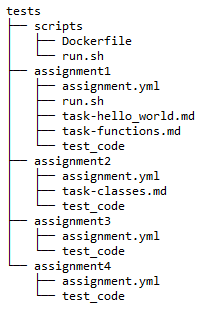
\includegraphics[scale=0.8]{photos/tests-repository-structure-tasks.PNG}
    \caption{Example of a tests repository with tasks}
    \label{fig:tests-repository-structure-tasks}
\end{figure}

\textbf{Pull Requests}

For every issue, group members are expected to solve them by creating a new branch and pull request.
QuickFeed should then support...
\begin{itemize}
    \item Returning automatic feedback in the form of a comment every time a student pushes to a pull request.
    \item Automatically assigning appropriate reviewers when students get a passing score on their code.
    Specifically one teacher and one other group member.
\end{itemize}

\section{Existing implementation}

An implementation has already been attempted for this project. % TODO: Ref here, and mention both names.
Before we can begin with a new one, we first have to decide which parts of it we want to use, and which to discard.
These parts are summarized in this section.

\subsection{SCM Expansion}
\label{sec:scm_expansion}

The SCM package has been expanded to support the following functions:

\begin{itemize}
    \item CreateIssue   - creates an issue on a repository.
    \item EditIssue - edits an issue on a repository.
    \item GetIssue  - retrieves an issue based on issue number and repository.
    \item GetIssues - retrieves all issues from a repository.
\end{itemize}

CreateIssue and EditIssue would prove useful, and are used with only minor adjustments to them.
The two other functions, centered around retrieving issues were not needed, but still used in earlier parts of the project when testing.

\subsection{Logic}

A lot of existing code was intended to handle the logic around managing tasks. 
In short, this code was meant to do determine when to create, edit or delete issues on GitHub.
The code did however not accomplish this in a functional manner.
This lead to the dilemma of whether to continue developing this faulty code, or simply start anew.
In the end, we decided that any attempt to fix the existing logic code would be more time consuming and confusing than simply starting fresh.

\subsection{Finding and Parsing Tasks}
\label{sec:parsing_tasks}

When a teacher pushes assignments to the \textit{tests} repository, QuickFeed will run the function UpdateFromTestsRepo.
In short, this function creates a local copy of the folder structure in \textit{tests}, and uses the \textit{assignment.yml} files within to create assignment data objects.
These are then used to update the database records for the relevant assignments.
Added as a part of this process, was code to also parse all task markdown files in \textit{tests}, and use their contents to create task data objects.

Additionally, a new field is created for the existing \textbf{Assignment} message, giving the associated data structure the capacity to hold a list of tasks.
This is used to have any assignment data object created by UpdateFromTestsRepo also contain all the task data objects for that assignment.
\begin{lstlisting}[caption={Modification to the Assignment message}, numbers=none]
repeated Task tasks = 13;  // Tasks associated with this assignment
\end{lstlisting}

To support parsing task markdown files, all \textit{task-*.md} files are expected to conform to a standard format.
The first line should start with the character sequence "\# <task title>", followed by by two new line characters.
Any following text there after will be treated as the task body or description.

Using this format, the function newTask creates a task data object from any task file.

\lstinputlisting[caption={Function that creates a task object from markdown content}, language=Golang, firstline=25, lastline=40]{code/tasks.go}

Going forward, the general approach to parsing and creating tasks is left as it is, with only minor changes to the existing code.

\section{Managing Tasks and Issues}

Having looked at what existing code we decided to keep, we continue by exploring the part of the project that was implemented first; how to manage tasks and issues.

As a general clarification, tasks are defined by the contents of the \textit{task-*.md} markdown files in \textit{tests}.
An issue on the other hand, is defined as any GitHub issue based on these tasks.
As an example, we can have a course with an assignment containing three tasks.
In this course, we also have five group repositories.
These three tasks should then be represented on all five group repositories as GitHub issues, giving us a total of 15 issues.
Tasks therefore function as a "benchmark" used to create issues.
In this thesis students can be referred to as solving both tasks and issues, which in essence means the same thing.

\subsection{Approach}

To support teachers creating, updating and deleting tasks, QuickFeed must have the capacity to handle these events.
For example, if a task is created, QuickFeed should create an issue based on it in every group repository within the relevant course.
Similarly, as tasks are updated or deleted, these changes must also be reflected in every issue created from them.
In short, we need to keep every issue in sync with its associated task.

To accomplish this, we keep a reference to every task and issue in QuickFeed's database.
The task database records are used to store a reference to what a given task looked like on the last push to \textit{tests}.
Doing so, we can compare it with every task parsed in UpdateFromTestsRepo, the function that finds and creates assignments and tasks based on the contents of \textit{tests}.
Furthermore, by storing a reference to every issue we create, they can be used when tasks are updated or deleted, to update and delete all issues associated with these tasks.

The process of synchronizing both tasks and issues is handled by the new function handleTasks, which is run as part of UpdateFromTestsRepo.
The function handleTasks, and the synchronization process in general, are further described in the following sections. 

To avoid confusion, we define the following distinctions for assignments and tasks.
\begin{itemize}
    \item TRtask - \textit{tests} repository task. Meaning any task represented by a \textit{task-*.md} markdown file in \textit{tests}.
    \item DBtask - database task. Meaning any task that refers to an existing task data record stored in the database.
    \item TRassignment - \textit{tests} repository assignment. Meaning any assignment represented by a folder and \textit{assignment.yml} file
    in \textit{tests}. 
    \item DBassignment - database assignment. Meaning any assignment referring to an existing stored assignment data record.
\end{itemize}

\subsection{Data Structures}
\label{sec:tasks-and-issues-data-structures}

To manage tasks and issues, two new messages are defined in the \textit{ag.proto} file: \textbf{Task} and \textbf{Issue}.
These are used to generate the data structures that are stored in the database.
% The resulting \textbf{Task} data structure is also used to created the task data objects described in Section \ref{sec:parsing_tasks}

\textbf{Task} is defined in code \ref{code:Task}.

\lstinputlisting[caption={Task message}, label={code:Task}, firstline=185, lastline=193]{code/ag.proto}

The title and body fields are defined by the contents of a task markdown file.
They are used to represent the title and body of any issue that is created from a given task.

% TODO: Should maybe describe the assignment message in background, how the assignment.yml file is parsed into it. See Hein review.
For an assignment, order is a number used to determine the order in which it is represented in a course.
It is set by a teacher in the \textit{assignment.yml} file, as described in Section \ref{sec:quickfeed-repository-structure}.
When creating a new task, keeping track of the corresponding assignment order is useful.
It allows us to associate tasks and assignments without explicitly knowing the assignment ID, so long as our scope is limited to just a single course.
A feature that will prove necessary.

The name field is used to associate TRtasks with DBtasks.
If a task file with the name \textit{task-hello\_world.md} is found within \textit{assignment1}, then its corresponding name will be assignment1/hello\_world.
This name is set when the task itself is parsed, as described in Section \ref{sec:parsing_tasks}.

Every TRtask and DBtask is represented by the data structure generated by this message.

\textbf{Issue} is defined in code \ref{code:Issue}.

\lstinputlisting[caption={Issue message}, label={code:Issue}, firstline=195, lastline=200]{code/ag.proto}

When compiled, the generated data structure is used to represent issues in QuickFeed.
The issueNumber and repositoryID fields let us hold a reference to every GitHub issue.

\subsection{Synchronizing Tasks}

As mentioned, we store references to tasks in the database.
When teachers push new or updated TRtasks to \textit{tests}, QuickFeed must create and update the existing DBtask records respectively.
Similarly, when a TRtask has been removed, its respective DBtask must also be deleted from the database.

These events are handled by the database method SynchronizeAssignmentTasks, which is run at the start of handleTasks.
SynchronizeAssignmentTasks is supplied with every TRassignment created by UpdateFromTestsRepo, each with their list of TRtasks.
They are then used to create the following mapping.
\begin{lstlisting}[caption={Task mapping}, language=Golang, label={code:task-mapping}, numbers=none, basicstyle=\ttfamily\footnotesize]
taskMap[assignmentOrder][taskName] = TRtask
\end{lstlisting}
This mapping allows us to loop through all DBassignment records in a course, and associate each of its DBtasks with a TRtask.

The process of synchronizing DBtasks is explained as follows.
For every DBtask in a DBassignment, check if it has the same name as any of the TRtasks.
If no match can be found for the DBtask, it must mean that the TRtask has been removed, and the task itself no longer exists.
The DBtask can therefore be safely deleted.
However, if there is a match for the DBtask, we check if its body or title differs from its TRtask counterpart.
If true, it must mean that the task has been updated, and if not, the task remains unchanged.
Furthermore, any TRtask that is not represented by a DBtask must represent a new task, and we therefore create a DBtask to represent it.

The main synchronization logic performed by SynchronizeAssignmentTasks is listed in code \ref{code:SynchronizeAssignmentTasks}.
Note that error handling has been removed for simplicity.

% TODO: Should find a font for the comments, that makes them smaller.
\begin{lstlisting}[caption={Task synchronization performed by SynchronizeAssignmentTasks}, 
                            language=Golang, label={code:SynchronizeAssignmentTasks}]
for _, DBassignment := range DBassignments {
	var DBtasks []*pb.Task
	tx.Find(&DBtasks, &pb.Task{AssignmentID: DBassignment.GetID()})
	for _, DBtask := range DBtasks {
		TRtask, ok := taskMap[DBassignment.Order][DBtask.Name]
		if !ok {
			// Existing task in database not among the supplied tasks to synchronize.
			tx.Delete(DBtask).Error
			DBtask.MarkDeleted()
			updatedTasks = append(updatedTasks, DBtask)
			
			// Find issues associated with the existing task and delete them
			var issues []*pb.Issue
			tx.Delete(issues, &pb.Issue{TaskID: DBtask.ID})
			continue
		}
		if DBtask.HasChanged(TRtask) {
			// Task has been changed and must be updated.
			DBtask.Title = TRtask.Title
			DBtask.Body = TRtask.Body
			updatedTasks = append(updatedTasks, DBtask)
			tx.Model(&pb.Task{}).
				Where(&pb.Task{ID: DBtask.GetID()}).
				Updates(DBtask).Error
		}
		delete(taskMap[DBassignment.Order], DBtask.Name)
	}

	// Find new tasks to be created for the current assignment
	for _, TRtask := range taskMap[DBassignment.Order] {
		TRtask.AssignmentID = DBassignment.ID
		createdTasks = append(createdTasks, TRtask)
	}
}
\end{lstlisting}

SynchronizeAssignmentTasks also returns the DBtasks it has created or updated, which which are used when synchronizing issues.

\subsection{Synchronizing Issues}

When synchronizing issues we must make sure to synchronize not only the issue database records, but also the GitHub issues themselves.

As mentioned, SynchronizeAssignmentTasks already determines the tasks that have been created, updated or deleted.
In fact, when it detects that a task has been deleted, it deletes not only the task but all associated issue records, as seen on Line 14 in code \ref{code:SynchronizeAssignmentTasks}.
Issue data records also never need to be updated, since they carry no other non-relational information than an issue number, which always remains static.
The only remaining database related synchronization for issues is therefore creating them.

The entire process of synchronizing issues happens in handleTasks, and is shown in Code \ref{code:handleTasks}.
\begin{lstlisting}[caption={Issue synchronization performed by handleTasks}, language=Golang, label={code:handleTasks}]
createdIssues := []*pb.Issue{}
for _, repo := range repos {
	if !repo.IsGroupRepo() {
		continue
	}
	repoCreatedIssues, err := createIssues(ctx, sc, course, repo, createdTasks)
	if err != nil {
		return err
	}
	createdIssues = append(createdIssues, repoCreatedIssues...)
	if err = updateIssues(ctx, sc, course, repo, updatedTasks); err != nil {
		return err
	}
}
// Create issues in the database based on issues created on the scm.
return db.CreateIssues(createdIssues)
\end{lstlisting}

In short, we use the created and updated DBtasks returned by SynchronizeAssignmentTasks, as arguments in createIssues and updateIssues respectively.
These functions use the SCM functions described in section \ref{sec:scm_expansion}.
Then, by looping through every course group repository GitHub issues are created and updated accordingly.
The function createIssues also returns a list of all the issues it created.
These are used at the end of the process to create issue database records.

It is worth mentioning that there is no description of how we delete GitHub issues in the above process.
To delete issues, we wanted to expand the SCM API to give it that capacity.
It turns out however, that GitHub's REST API does not support deleting issues.
An alternative could have been to use GraphQL, a query language for API's, but instead we went for a simpler solution.
In place of deleting issues, they are closed, and their title and body are inserted with a statement indicating that the associated task has been deleted.

\section{Managing Pull Requests}

Having implemented support for tasks and issues, we must now do the same for pull requests.

\subsection{Pull Request Data Structure}
\label{sec:pull-request-data-structure}

To manage pull requests we need a data structure to represent them.
For this purpose, the \textbf{PullRequest} message is created.

\begin{lstlisting}[caption={PullRequest message}]
message PullRequest {
    enum Stage {
        NONE    = 0;
        DRAFT   = 1;
        REVIEW  = 2;
        APPROVED = 3;
    }
    uint64 ID                   = 1;
    uint64 externalRepositoryID = 2; // Represents the external repository ID
    uint64 taskID               = 3; // Foreign key
    uint64 issueID              = 4; // Foreign key
    uint64 userID               = 5; // The user who owns this PR
    uint64 commentID            = 6; // GitHub ID of the comment used for automatic feedback
    string sourceBranch         = 7; // The source branch for this pull request
    uint64 number               = 8; // Pull request number
    Stage stage                 = 9;
}
\end{lstlisting}

% TODO: Describe this message, and why certain fields are needed.
% TODO: Describe why linking the issue is important, i.e. we can delete the issue data record, and the issue is closed on GitHub.

\subsection{Creating Pull Requests}

As students create pull requests to solve issues/tasks, we must make sure that a pull request record is created and stored internally to represent them.
Doing so allows us to keep track of which student is solving what task, who should be assigned to review the pull request, and more.
This section describes how this is implemented.

In section \ref{sec:creating-pull-requests} we decided to have students manually create pull requests.
To accommodate this feature, QuickFeed must react to the pull requests being opened.
Expanding QuickFeed to also handle pull request related webhooks, allows us to do just that.

Specifically, when a pull request is opened the handlePullRequestOpened function is run.
It will check if a pull request is legitimate, i.e. it was created on a group repository and linked to the correct issue.
If successful, the function creates a new record to represent it, by using the data in the event payload, and then stores it in the database.

Associating a pull request to an issue requires that the student themselves explicitly do so.
GitHub allows you to link issues to pull requests on their creation, by inserting a reference to them in the pull request body.
Doing so, we thought that the linked issue would also be part of the webhook payload, however, this turned out to be incorrect.
Instead we have to parse the issue number from the pull request body itself, as shown below.
% TODO: Should get code from file instead, when everything has been finalized.
\begin{lstlisting}[caption={The getLinkedIssue function}, language=Golang]
func getLinkedIssue(body string) (uint64, error) {
	if count := strings.Count(body, "#"); count != 1 {
		return 0, errors.New("pull request body does not contain exactly one '#' character")
	}
	subStrings := strings.Split(body, "#")
	issueNumber, err := strconv.Atoi(subStrings[len(subStrings)-1])
	if err != nil {
		return 0, fmt.Errorf("failed to parse issue number from pull request body: %w", err)
	}
	return uint64(issueNumber), nil
}
\end{lstlisting}

This solution somewhat limits the possible contents of a pull request body.
For example, students must make sure only to use one "\#" character for the function to succeed.
This is further discussed in section .% TODO: Ref to relevant discussion section.

\subsection{Closing Pull Requests}

When students close and merge pull requests---ideally when they are supposed to---QuickFeed must also act accordingly.
Again, we use webhooks to listen to pull request closed events, and single out those that are relevant to QuickFeed.
Relevant in this context, is any event for a pull request that already exist in QuickFeed's database, i.e. they were created as part of the process described in the above section.
Events for pull requests that are closed, but not merged, can also be filtered out, as these constitute an incorrect close.
If students do happen to close pull requests like this, a working state can be restored by the student, simply by reopening it.
QuickFeed doing nothing in these cases is therefore the simplest solution.

Assuming that the event is valid, there are two possible outcomes.
Either the pull request is approved, and it and its associated issue can safely be deleted from the database.
Or, it has been closed and merged by a student without being explicitly approved by a teacher.
If this happens, QuickFeed must have the capacity to restore a working state for the issue/task in question.
To handle these situations, QuickFeed deletes only the pull request and not the issue record.
This way, a student doing an incorrect merge can simply reopen the issue that was closed, and then create a new pull request to represent it.
Thereby restoring a working state with little QuickFeed involvement.

\section{Scoring Tasks}

To allow for both automatic and manual feedback, we need a way to score tasks.
Delivering automatic feedback requires us to do so solely on the tests associated with any given task.
Manual feedback on the other hand, needs some sort of task related score to determine when to assign reviewers.
Currently, QuickFeed only tests and scores student code based on an assignment as a whole.
Having it do so on a per task basis therefore seems like a necessity to fulfill our goals.

QuickFeed's ci package is fundamentally designed to test assignments, therefore rewriting it to support tasks would be challenging.
Any solution might also not be backwards compatible.
To implement our features though, QuickFeed does not need to test task related code, only score it.
As such, we can instead complement the score package to support this functionality.

% TODO: Need to describe the following changes further, and use code samples
Doing so turned out to be pretty straight forward.
First, the score message described in section \ref{sec:the-score-package} is modified to also include a task name field.
Doing so, gives us a direct reference to the task a given score is associated with.
Furthermore, to support teachers adding task specific tests, two new variants of the existing Add and AddSub methods are created.
These allow teachers to specify the task name a test should be a part of.
Finally, to generate a task specific total score, QuickFeed simply sums over the scores that have that task's name.

It should be noted that when referring to a task name in the context of the score package, we mean the local task name.
The local task name differs from the regular one by omitting the assignment name prefix.
As an example, a task with the name \textit{assignment1/hello\_world} will have the local name \textit{hello\_world}.
This was primarily done to make the process of associating tests and tasks more intuitive for the teachers doing so.

With these changes implemented, we can generate a score from 0 - 100 for specific tasks, just as is already possible for entire assignments.

\section{Manual Feedback}

Having implemented QuickFeed support for scoring tasks in the previous section, these features can now be used to facilitate manual review.
In short, our approach is to assign one student and teacher reviewer to a pull request once a passing score is reached.
This passing score limit is the same as the assignment score limit.

Checking whether a task is passed or not must be done every time a student pushes to a group repository.
QuickFeed already has a function that handles these push events, and we can therefore manage all review assignment related logic there.

\subsection{Assigning Reviewers}
\label{sec:assigning-reviewers}

To handle pushes to non-default branches in group repositories we implemented the handlePullRequestPush function.
Its primary job is to attempt to find a pull request that is associated with a given branch push.
In the event payload, there is information about both the branch and the repository that was pushed to.
Using these, QuickFeed queries the database for the specific pull request that is associated with them.

If a pull request exists for the repository and remote branch, it is used to retrieve the task associated with it.
Doing so allows us to get the specific task name, which can then be used to retrieve the task specific total score.
Finally, if this score is greater than the score limit, the assignment process can begin.

Before assigning reviewers there are a few things that have to be accounted for.
First of, we need to make sure not to assign the same reviewers over and over.
To illustrate, we do not want one teacher to review every pull request in a course, with the rest of the teachers not being assigned to review anything.
Similarly, having one group member review every pull request within a group is also unwanted.
Secondly, the owner of a pull request must not be assigned as its reviewer.

To tackle the first problem, we use two maps, one for teachers and one for group members, to facilitate in-memory storage of every reviewer.
Specifically, these maps track the total amount of times every reviewer has been assigned to a pull request.
They are described as follows, and are as shown, in fact maps of maps.

\begin{lstlisting}[caption={Maps used to store review counts}, language=Golang, numbers=none, basicstyle=\ttfamily\footnotesize]
teacherReviewCounter[courseID][userID]  = count
groupReviewCounter[groupID][userID]     = count
\end{lstlisting}

These are then used as arguments in the function getNextReviewer.
getNextReviewer's purpose is to find, amongst the supplied users, the one that has the least amount of total reviews, and then return said user.
By supplying it with all course teachers or a group's members, it finds the next eligible teacher or student reviewer respectively.
To tackle the second problem mentioned earlier, we make sure to to not include the pull request owner in the user list.
% TODO: Should get code from file instead, when everything has been finalized.
\begin{lstlisting}[caption={The getNextReviewer function}, language=Golang]
func getNextReviewer(ID uint64, users []*pb.User, reviewCounter map[uint64]map[uint64]int) (*pb.User, error) {
	if len(users) == 0 {
		return nil, errors.New("list of users is empty")
	}
	reviewerMap, ok := reviewCounter[ID]
	if !ok {
		// If a map does not exist for a given ID we create it,
		// and return the first user.
		reviewCounter[ID] = make(map[uint64]int)
		reviewCounter[ID][users[0].GetID()] = 1
		return users[0], nil
	}
	userWithLowestCount := users[0]
	lowestCount := reviewerMap[users[0].GetID()]
	for _, user := range users {
		count, ok := reviewerMap[user.GetID()]
		if !ok {
			// If the user is not present in the review map,
			// then they are returned as the next reviewer.
			reviewerMap[user.GetID()] = 1
			return user, nil
		}
		if count < lowestCount {
			userWithLowestCount = user
			lowestCount = count
		}
	}
	reviewerMap[userWithLowestCount.GetID()]++
	return userWithLowestCount, nil
}
\end{lstlisting}

In order to actually assign reviewers to a GitHub pull request, the SCM API is expanded with the function RequestReviewers.
It is supplied with the GitHub login usernames of the retrieved reviewers.
If successful, the entire process is finished by updating the pull request stage to review, signaling that it is now being reviewed.

\subsection{Approving Pull Requests}

Having described how reviewers are assigned to pull requests in the previous section, this section explores what happens when teachers approve them.

The function handlePullRequestReview handles everything related to pull request reviews.
It is triggered by pull request review related webhooks, and uses the accompanying payload to find the relevant pull request record.
If one exists, it attempts to find the user that posted the review.
The reason why the specific reviewer is needed, is because we must make sure that the review is from an actual teacher.
Otherwise, the group member that was assigned to review could also internally approve the pull request.
So, as long as the review is from a teacher, the pull request stage is updated to approved, meaning that it can be safely merged.

\section{Automatic Feedback}

Using QuickFeed's new capacity to score tasks, we implemented support for manual feedback on pull requests.
This new capacity also allows for automatic feedback on the same pull requests.

The approach is to use a single comment on a student's pull request to automatically publish test results from their latest commit.
This comment must be updated every time the student pushes to their pull request, and as such we can therefore use the function handlePullRequestPush.
A function that is used to manage all non-default branch pushes to group repositories, as described in Section \ref{sec:assigning-reviewers}.

\subsection{Formatting Feedback Comments}

To create the feedback comment itself, we must format one based on the test results for a given push.
For this purpose, we create the function CreateFeedbackComment.

The general idea is to use the task specific scores, as part of the test results for an assignment, to generate a table.
For every task specific test, we can describe its received score, the weight of the test, and how much the results from that test counts towards the total score.
GitHub lets you create tables in comments by using a special string formatting.
With this in mind, CreateFeedbackComment is described in Code \ref{code:CreateFeedbackComment}.

\begin{lstlisting}[caption={The CreateFeedbackComment function}, label={code:CreateFeedbackComment}, language=Golang]
func CreateFeedbackComment(results *score.Results, task *pb.Task, assignment *pb.Assignment) string {
	body := "## Test results from latest push\n"
	body += "| Test Name | Score | Weight | % of Total |\n"
	body += "| :-------- | :---- | :----- | ---------: |\n"

	for _, score := range results.Scores {
		if score.TaskName != task.LocalName() {
			continue
		}
		percentageScore := (float64(score.Score) / float64(score.MaxScore)) * (float64(score.Weight) / results.TotalTaskWeight(task.LocalName()))
		body += fmt.Sprintf("| %s | %d/%d | %d | %.2f%% |\n", score.TestName, score.Score, score.MaxScore, score.Weight, percentageScore*100)
	}
	body += fmt.Sprintf("| **Total** | | | **%d%%** |\n\n", results.TaskSum(task.LocalName()))
	body += fmt.Sprintf("Once a total score of %d%% is reached, reviewers are automatically assigned.\n", assignment.GetScoreLimit())
	return body
}
\end{lstlisting}

To illustrate, we can supply CreateFeedbackComment with the results, task and assignment described in Code \ref{code:sample-CreateFeedbackComment}.
\begin{lstlisting}[caption={Example of a CreateFeedbackComment run}, label={code:sample-CreateFeedbackComment}, language=Golang]
results := &score.Results{
	Scores: []*score.Score{
		{TestName: "Test1", TaskName: "1", Score: 5, MaxScore: 7, Weight: 2},
		{TestName: "Test2", TaskName: "1", Score: 3, MaxScore: 9, Weight: 3},
		{TestName: "Test3", TaskName: "1", Score: 8, MaxScore: 8, Weight: 5},
		{TestName: "Test4", TaskName: "1", Score: 2, MaxScore: 5, Weight: 1},
		{TestName: "Test5", TaskName: "1", Score: 5, MaxScore: 7, Weight: 1},
		{TestName: "Test6", TaskName: "2", Score: 5, MaxScore: 7, Weight: 1},
		{TestName: "Test7", TaskName: "3", Score: 5, MaxScore: 7, Weight: 1},
	},
}
CreateFeedbackComment(results, &pb.Task{Name: "lab1/1"}, 
                        &pb.Assignment{Name: "lab1", ScoreLimit: 80})
\end{lstlisting}

The resulting comment body in Figure \ref{fig:feedback-comment} is then created.
Note that the tests with name \textit{Test6} and \textit{Test7} are omitted from the table, because they are not associated with the task supplied to CreateFeedbackComment.
I.e. they do not have the same name.

\begin{figure}[ht]
    \centering
    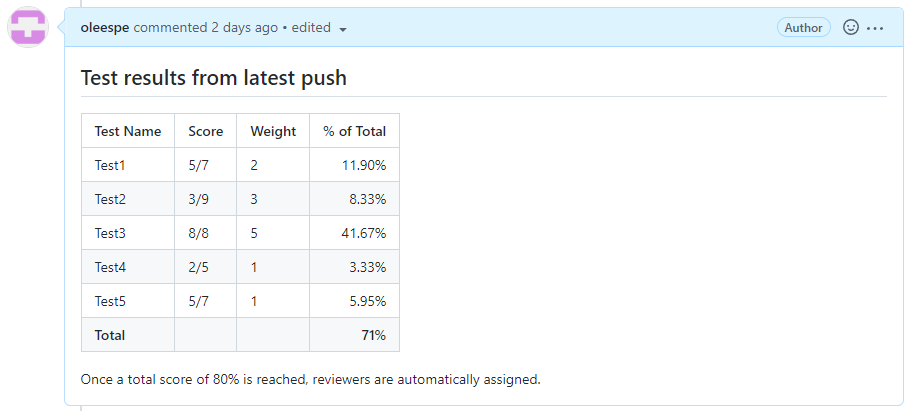
\includegraphics[width=\textwidth]{photos/feedback-comment.PNG}
    \caption{Feedback comment on a pull request}
    \label{fig:feedback-comment}
\end{figure}

\subsection{Publishing Feedback Comments}

To actually publish the feedback comments to a GitHub pull request, we again expand the SCM API.
The function CreateIssueComment is used to create the comments, while EditIssueComment updates existing ones.
The reason for using "Issue" in the function names instead of "PullRequest", is because GitHub treats pull requests as issues with code.
GitHub API calls to comment on issues and pull requests is therefore the same.

The first time a student pushes to a pull request, we use CreateIssueComment to create the initial comment.
CreateIssueComment returns the ID of the comment that was created, which is then stored as a field on the relevant pull request record.
Any subsequent pushes to the same pull request will then instead use EditIssueComment, which takes that ID as an argument.
Doing so, only one comment is present on the student's pull request.